% Created 2017-07-01 lø 22:29
% Intended LaTeX compiler: pdflatex
\documentclass{article}
               \usepackage{listings}
\usepackage{color}
\usepackage{amsmath}
\usepackage{array}
\usepackage[T1]{fontenc}
\usepackage{natbib}
               \usepackage[top=3cm, bottom=3cm, left=3cm, right=3cm]{geometry}

\lstset{
keywordstyle=\color{blue},
commentstyle=\color{red},stringstyle=\color[rgb]{0,.5,0},
literate={~}{$\sim$}{1},
basicstyle=\ttfamily\small,
columns=fullflexible,
breaklines=true,
breakatwhitespace=false,
numbers=left,
numberstyle=\ttfamily\tiny\color{gray},
stepnumber=1,
numbersep=10pt,
backgroundcolor=\color{white},
tabsize=4,
keepspaces=true,
showspaces=false,
showstringspaces=false,
xleftmargin=.23in,
frame=single,
basewidth={0.5em,0.4em},
}

\usepackage[utf8]{inputenc}
\usepackage[T1]{fontenc}
\usepackage{graphicx}
\usepackage{grffile}
\usepackage{longtable}
\usepackage{wrapfig}
\usepackage{rotating}
\usepackage[normalem]{ulem}
\usepackage{amsmath}
\usepackage{textcomp}
\usepackage{amssymb}
\usepackage{capt-of}
\usepackage{hyperref}
\author{Brice Ozenne}
\date{\today}
\title{Splines vs. polynomes for fitting non-linear relationships}
\hypersetup{
 pdfauthor={Brice Ozenne},
 pdftitle={Splines vs. polynomes for fitting non-linear relationships},
 pdfkeywords={},
 pdfsubject={},
 pdfcreator={Emacs 24.5.1 (Org mode 9.0.4)}, 
 pdflang={English}}
\begin{document}

\maketitle
\tableofcontents

\bigskip

\emph{Note:} this is document is inspired from \url{http://stackoverflow.com/questions/15837763/b-spline-confusion}

\clearpage

\section{Simulate data}
\label{sec:org582433f}
\lstset{language=r,label= ,caption= ,captionpos=b,numbers=none,otherkeywords={}, deletekeywords={}}
\begin{lstlisting}
library(splines)
library(data.table)
library(ggplot2)
library(mgcv)

set.seed(1)
n <- 400

x <- 0:(n-1)/(n-1)
dt <- data.table(X = x,
		 Ytrue =  0.2*x^11*(10*(1-x))^6+10*(10*x)^3*(1-x)^10)
dt[,Y := Ytrue + rnorm(n, 0, sd = 0.5)]
\end{lstlisting}


\section{Prepare data with non linear transformations of X}
\label{sec:orgb92dd9d}
\lstset{language=r,label= ,caption= ,captionpos=b,numbers=none,otherkeywords={}, deletekeywords={}}
\begin{lstlisting}
dt[,X2 := X^2]
dt[,X3 := X^3]
dt[,X4 := X^4]
dt[,X5 := X^5]
dt[,X6 := X^6]

Xknots <- c(0.2, 0.5, 0.7)
SplineTempo <- bs(dt$X, knots = Xknots)
dt <- cbind(dt, setNames(as.data.frame(SplineTempo), paste0("S",1:ncol(SplineTempo))))
\end{lstlisting}

\clearpage

\section{Fit models}
\label{sec:org038f4c4}
\lstset{language=r,label= ,caption= ,captionpos=b,numbers=none,otherkeywords={}, deletekeywords={}}
\begin{lstlisting}
lmPoly <- lm(Y ~ X + X2 + X3 + X4 + X5 + X6, data = dt)

lmSpline <- lm(Y ~ bs(x, knots = c(0.2, 0.5, 0.7)), data = dt)

lmSplineI <- lm(Y ~ S1 + S2 + S3 + S4 + S5 + S6, data = dt)
range(coef(lmSpline)-coef(lmSplineI)) # same as lmSpline

autoSpline <- gam(Y ~ s(X), data = dt)
\end{lstlisting}

\begin{verbatim}
[1] 0 0
\end{verbatim}

Residual degree of freedom:
\lstset{language=r,label= ,caption= ,captionpos=b,numbers=none,otherkeywords={}, deletekeywords={}}
\begin{lstlisting}
c(df.residual(lmPoly),df.residual(lmSpline), df.residual(autoSpline))
\end{lstlisting}

\begin{verbatim}
[1] 393.0000 393.0000 390.0559
\end{verbatim}

\section{Extract the fitted values}
\label{sec:org46df0fb}
\lstset{language=r,label= ,caption= ,captionpos=b,numbers=none,otherkeywords={}, deletekeywords={}}
\begin{lstlisting}
seqX <- seq(min(dt$X), max(dt$X), length = 100)

dt2 <- data.table(Y = dt$Y, X = dt$X, type = "observed")

predPoly <- predict(lmPoly, newdata = data.frame(X = seqX, X2 = seqX^2, X3 = seqX^3, X4 = seqX^4, X5 = seqX^5, X6 = seqX^6))
dt2 <- rbind(dt2, data.frame(Y = predPoly, X = seqX, type = "poly"))

predSpline <- predict(lmSpline, newdata = data.frame(x = seqX))
dt2 <- rbind(dt2, data.frame(Y = predSpline, X = seqX, type = "spline"))

predGam <- predict(autoSpline, newdata = data.frame(X = seqX))
dt2 <- rbind(dt2, data.frame(Y = predGam, X = seqX, type = "gam"))
\end{lstlisting}

\section{Display fit}
\label{sec:orga713274}

\lstset{language=r,label= ,caption= ,captionpos=b,numbers=none,otherkeywords={}, deletekeywords={}}
\begin{lstlisting}
ggbase <- ggplot(dt2[dt2$type == "observed",], aes(x = X, y = Y)) + geom_point()
ggbase <- ggbase + geom_line(data = dt2[dt2$type != "observed",],
			     aes(x = X, y = Y, group = type, color = type),
			     size = 2)
 ggbase <- ggbase + theme(text = element_text(size=30))
\end{lstlisting}

\begin{center}
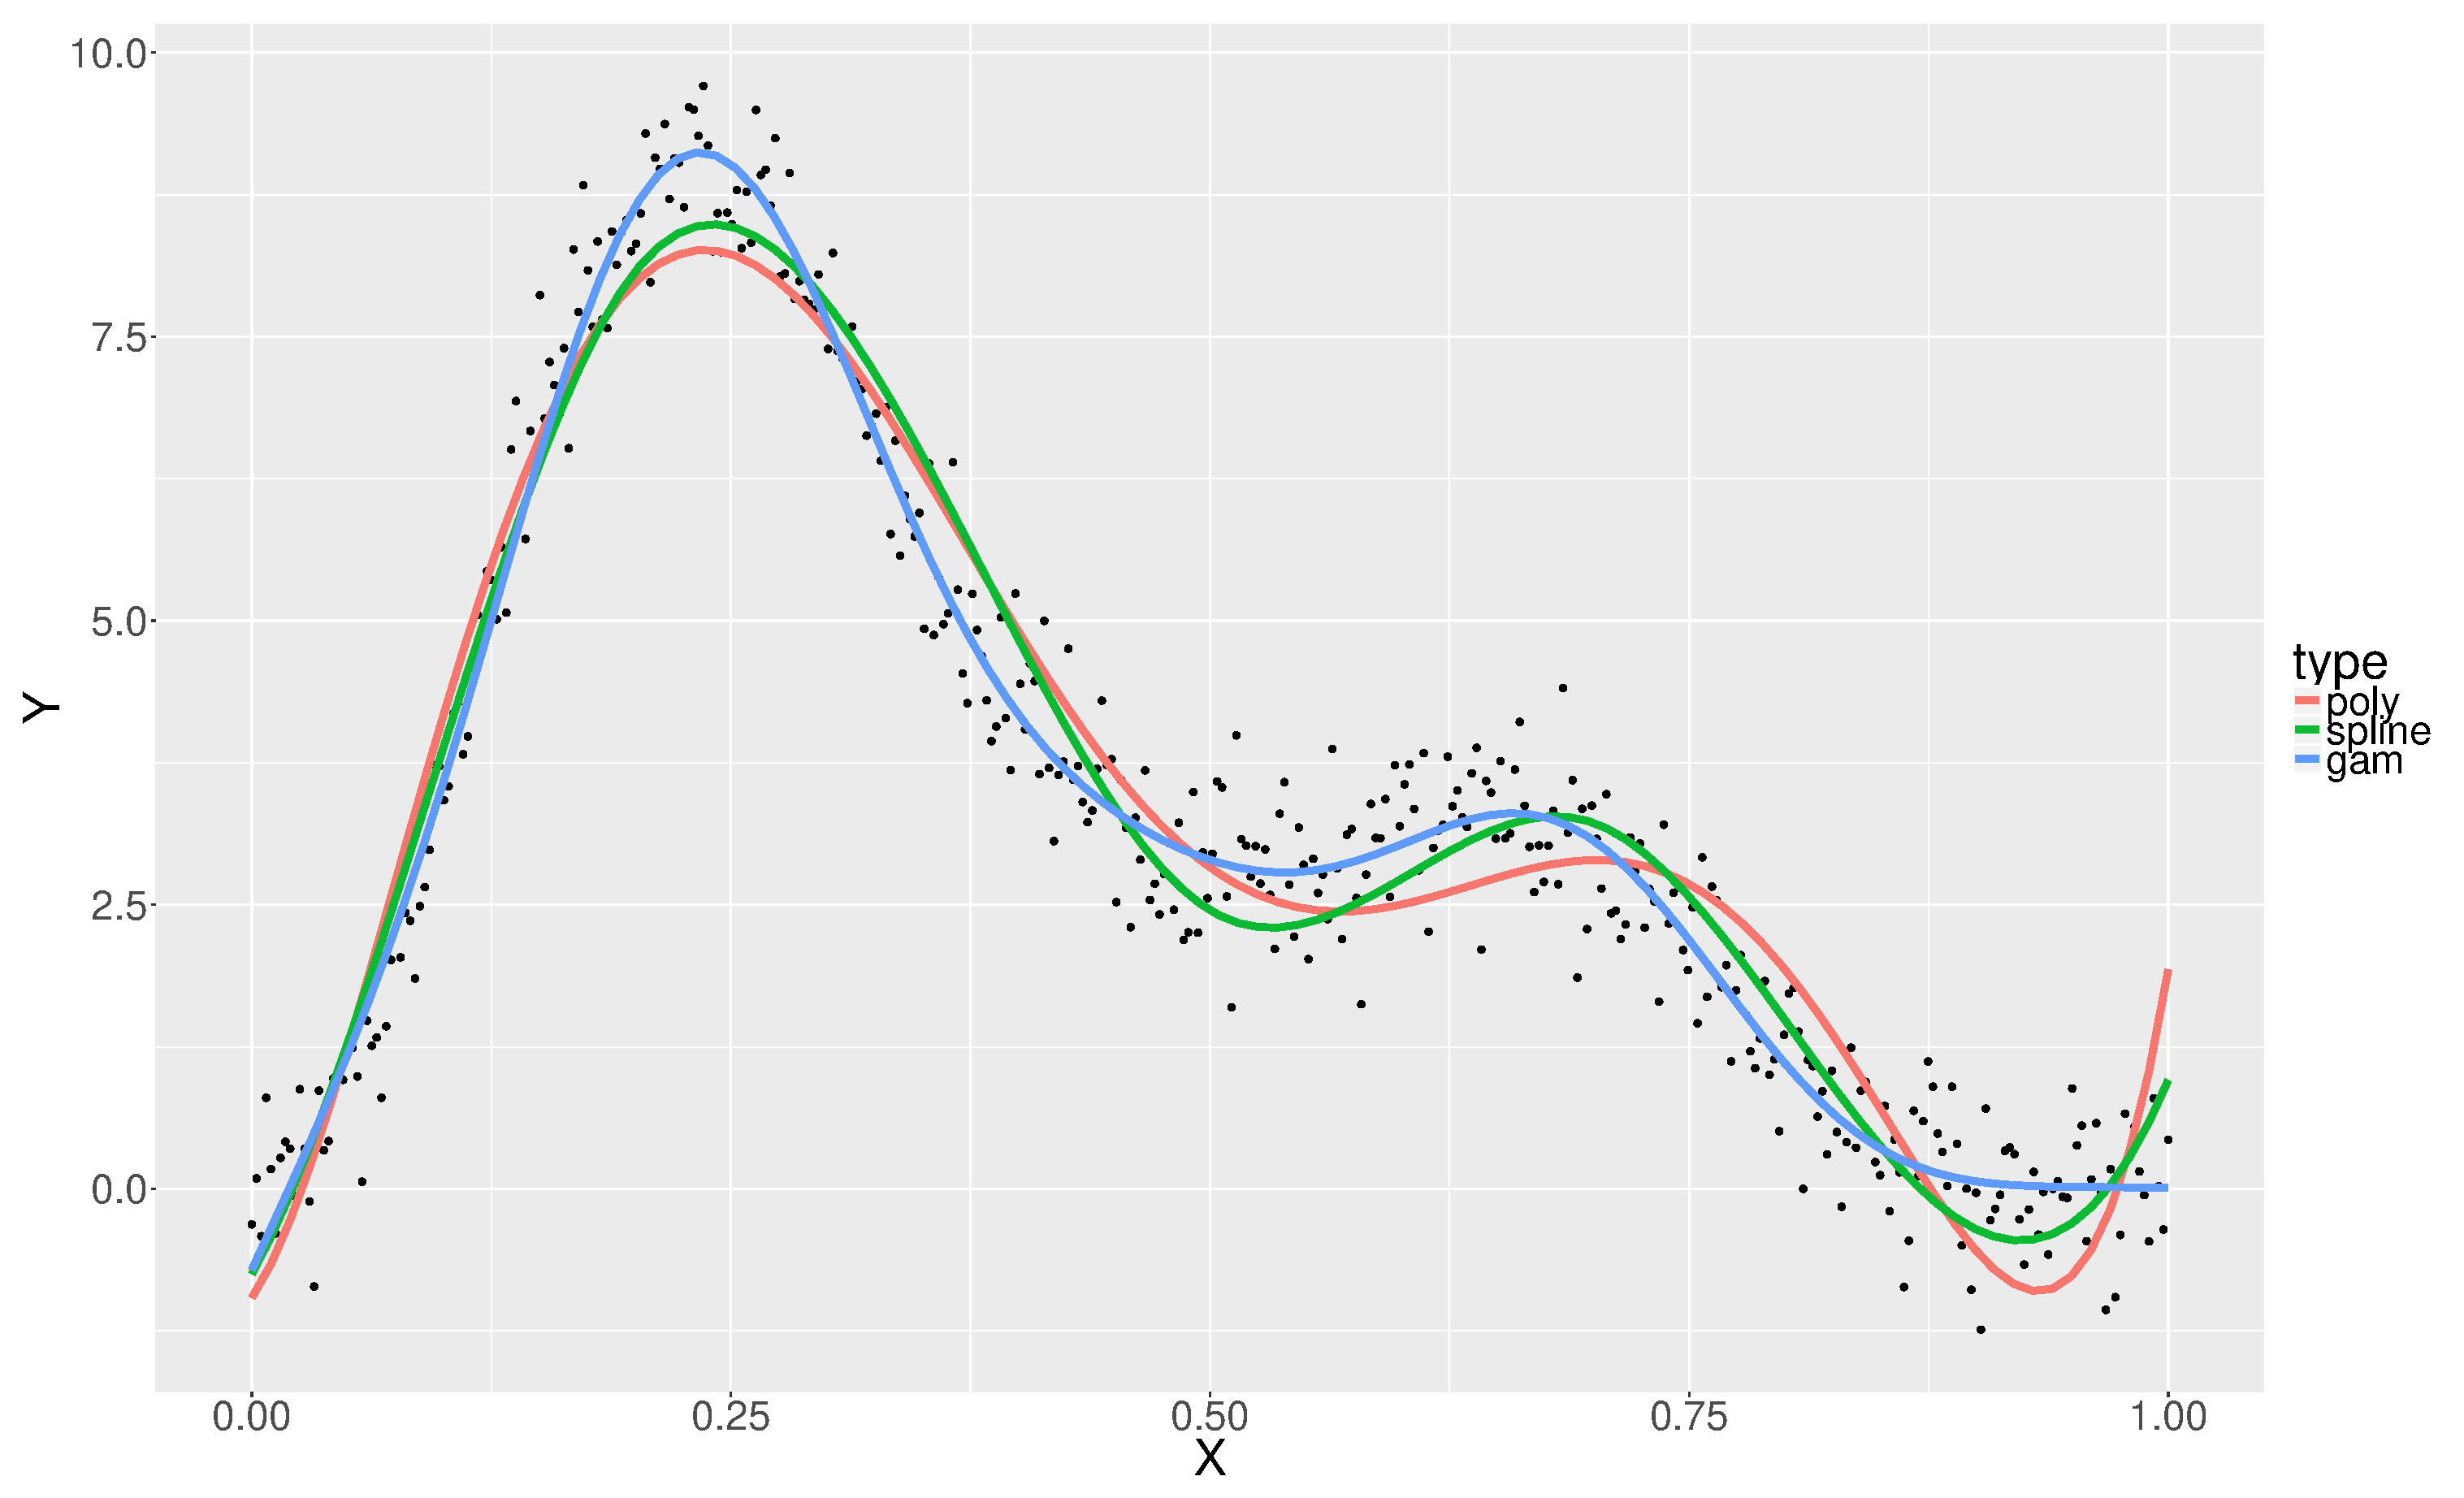
\includegraphics[clip=true, trim=0cm 0cm 0cm 0cm,width=1\textwidth]{./comparaison.eps}
\end{center}


Splines give a better fit compared to a 3rd order polynomial when the knots are correctly placed
\end{document}